\documentclass[twocolumn,10pt]{article}
\setlength\textwidth{6.875in}
\setlength\textheight{8.875in}
% set both margins to 2.5 pc
\setlength{\oddsidemargin}{-0.1875in}% 1 - (8.5 - 6.875)/2
\setlength{\evensidemargin}{-0.1875in}
\setlength{\marginparwidth}{0pc}
\setlength{\marginparsep}{0pc}%
\setlength{\topmargin}{0in} \setlength{\headheight}{0pt}
\setlength{\headsep}{0pt}
\setlength{\footskip}{37pt}%
%\setlength{\columnsep}{0.3125in}
%\setlength{\columnwidth}{3.28125in}% (6.875 - 0.3125)/2 = 3.28125in
\setlength{\parindent}{1pc}
\newcommand{\myMargin}{1.00in}
\usepackage[top=\myMargin, left=\myMargin, right=\myMargin, bottom=\myMargin, nohead]{geometry}
\usepackage{epsfig,graphicx}
\usepackage{palatino}
\usepackage{fancybox}
\usepackage{url}
\usepackage{ctex}
\usepackage[procnames]{listings}

% "define" Scala
\usepackage[T1]{fontenc}  
\usepackage[scaled=0.82]{beramono}  
\usepackage{microtype} 

\sbox0{\small\ttfamily A}
\edef\mybasewidth{\the\wd0 }

\lstdefinelanguage{scala}{
  morekeywords={abstract,case,catch,class,def,%
    do,else,extends,false,final,finally,%
    for,if,implicit,import,match,mixin,%
    new,null,object,override,package,%
    private,protected,requires,return,sealed,%
    super,this,throw,trait,true,try,%
    type,val,var,while,with,yield},
  sensitive=true,
  morecomment=[l]{//},
  morecomment=[n]{/*}{*/},
  morestring=[b]",
  morestring=[b]',
  morestring=[b]"""
}

\usepackage{color}
\definecolor{dkgreen}{rgb}{0,0.6,0}
\definecolor{gray}{rgb}{0.5,0.5,0.5}
\definecolor{mauve}{rgb}{0.58,0,0.82}

% Default settings for code listings
\lstset{frame=tb,
  language=scala,
  aboveskip=3mm,
  belowskip=3mm,
  showstringspaces=false,
  columns=fixed, % basewidth=\mybasewidth,
  basicstyle={\small\ttfamily},
  numbers=none,
  numberstyle=\footnotesize\color{gray},
  % identifierstyle=\color{red},
  keywordstyle=\color{blue},
  commentstyle=\color{dkgreen},
  stringstyle=\color{mauve},
  frame=single,
  breaklines=true,
  breakatwhitespace=true,
  procnamekeys={def, val, var, class, trait, object, extends},
  procnamestyle=\ttfamily\color{red},
  tabsize=2
}

\lstnewenvironment{scala}[1][]
{\lstset{language=scala,#1}}
{}
\lstnewenvironment{cpp}[1][]
{\lstset{language=C++,#1}}
{}
\lstnewenvironment{bash}[1][]
{\lstset{language=bash,#1}}
{}
\lstnewenvironment{verilog}[1][]
{\lstset{language=verilog,#1}}
{}



\lstset{frame=, basicstyle={\footnotesize\ttfamily}}

\newcommand{\todo}[1]{\emph{TODO: #1}}
\newcommand{\comment}[1]{\emph{Comment: #1}}

% uncomment following for final submission
\renewcommand{\todo}[1]{}
\renewcommand{\comment}[1]{}

\newenvironment{commentary}
{ \vspace{-0.1in}
  \begin{quotation}
  \noindent
  \small \em
  \rule{\linewidth}{1pt}\\
}
{
  \end{quotation}
}

% \newenvironment{kode}%
% {\footnotesize
%  %\setlength{\parskip}{0pt}
%   %\setlength{\topsep}{0pt}
%   %\setlength{\partopsep}{0pt}
%  \verbatim}
% {\endverbatim 
% %\vspace*{-0.1in}
%  }

% \newenvironment{kode}%
% {\VerbatimEnvironment
% \footnotesize\begin{Sbox}\begin{minipage}{6in}\begin{Verbatim}}%
% {\end{Verbatim}\end{minipage}\end{Sbox}
% \setlength{\fboxsep}{8pt}\fbox{\TheSbox}}

% \newenvironment{kode}
% {\begin{Sbox}
% \footnotesize
% \begin{minipage}{6in}
%   %\setlength{\parskip}{0pt}
%   %\setlength{\topsep}{0pt}
%   %\setlength{\partopsep}{0pt}
%   \verbatim}
% {\endverbatim 
% \end{minipage}
% \end{Sbox} 
% \fbox{\TheSbox}
%  %\vspace*{-0.1in}
%  }

\title{多发射乱序CPU的RTL级实现与验证}
\author{ 开题报告\\
{\tt 周盈坤} \\
{\tt  zhouyingkun15@mails.ucas.ac.cn}
}
\date{\today}

\newenvironment{example}{\VerbatimEnvironment\begin{footnotesize}\begin{Verbatim}}{\end{Verbatim}\end{footnotesize}}
\newcommand{\kode}[1]{\begin{footnotesize}{\tt #1}\end{footnotesize}}

\def\code#1{{\tt #1}}

\def\note#1{\noindent{\bf [Note: #1]}}
%\def\note#1{}

\begin{document}
\maketitle{}

% TODO: default
% TODO: enum yields Bits
% TODO: why hardware construction languages

\section{opening}
\begin{commentary}
	计算机领域,体系结构者扮演的是上帝的角色。上帝造万物、制规律,但却察觉不到。用户不会关心在程序的背后何种指令是按照何种方式被执行,只会在乎在计算机世界里跑的应用程序如否满足自己的需求,是否流畅。
	
	操作体统犹如国王,国王管理着国家。国王即天子,和上帝ISA紧紧绑定。当今世界的三大国家的国王为Windows, MacOS, Linux. 国王有着极大的威严,号令着所有在这个国家的领域上运行的程序。如果需要时不时跨国,便可体会到不同国度的差异。
	
	普通软件程序犹如国家的臣民和机构,它们必须遵从国家的规章制度,服从国王调度,涉及到关键资源的操作,必须上报国家,由国家安排与分配,跨国公司也概莫能外。
	
	编译器则是使者,无论是王公贵族还是黎明百姓,都需要经由它来与上帝沟通,使之从高级语言转化为机器码。
\end{commentary}
本科阶段没有发论文的打算,一是体系结构这个领域十年磨一剑,仅凭本科毕设估计很难有成色;二是希望在本科阶段参与和体系结构、操作系统、编译原理有关的基础性工作,打好以后研究的基础。

曾与张科老师的交流中他问过这样的毕设工作有什么用,我倒觉得讲求实用性应该是建立在不断完善自己的学术工程素养基础之上的。也曾与汪文祥老师沟通过,他提出首先这个毕设的题目是偏重于工程实现的,论文方面不一定出彩;其次工作量大,不一定能够完成。所以要做好心理准备并一步步脚踏实地去完成毕设的工作。

\textbf{key word: }RISC-V, MIPS, CPU, out-of-order,multi-issue

\section{background \& the state of art}
乱序多发射的CPU是通往高性能处理器的必经之路,Intel、AMD、ARM都应经有了成熟的技术。一个典型的代表就是ARM Cortex A53。作为一个双发射8级静态调度的处理器核,面积很小,功耗很低,SPEC2000 INT base能够达到423分/GHz%TODO
. 但是另外一方面,乱序多发射的设计并不容易,而且比设计更加困难的是调试,如何保证复杂执行的CPU能够有条不紊,毫无错误的运行比如像Linux操作系统这样的大型软件更是难上加难。所幸前有Alpha的技术报告,后有BOOM的开源实现可供参考,而BOOM背后更是有整个RISC-V的开源生态。RISC-V作为近些年在总结了前人ISA设计中的利弊的基础上推出的一套设计清晰,干净整洁而优雅的开源ISA,大受学术界工业界的欢迎。鉴于其日臻完善的开源的开发调试工具,有如下考虑方案:
\begin{enumerate}
	\item UC, Berkeley 开发的高级硬件描述语言Chisel对单一时钟,同步复位的电路逻辑的刻画效率比verilog更高,而且对于可综合电路的描述能够做到和verilog同样的精确,故而完全可以采用Chisel进行毕设CPU的设计开发。
	\item 可以参考借鉴开源的BOOM代码实现。
	\item 可以学习借用RISC-V开源调试工具与手段。
	\item 可以低成本地在FPGA平台上的运行目前RISC-V开源的整套以Linux为首的软件栈。
\end{enumerate}

综上,计划的第一步是实现一个基于RISC-V ISA的乱序双发射的CPU,调试完毕能够跑通简单的测试程序,但深知这绝非易事。接着在时间允许的情况下做操作系统的移植,继而能够支持多核。注意到一开始的设计必须考虑到微结构和ISA之间的解耦合,这样将RISC-V改成MIPS工作量会降低很多。得到MIPS版本的CPU目的在于采用相同的微结构可以客观的对比两个ISA的优劣。同时作为工作的非常重要的一部分,性能的优化和设计空间的搜索分析必不可少,奢望能够在跑相同benchmark的情况下持平甚至超过ARM的Cortex A53的水平。

\section{language and representation}
\subsection{Verilog}
Verilog是目前流行通用的硬件描述语言,表现能力强,语言设计参考的是C语言而且最开始设计出来是用作仿真的,因而有很多用于仿真的语法。但是真正可以用于综合电路的语言并不多,比较常规的有组合逻辑的assign语句,时序逻辑的时钟上升沿出发的同步电路逻辑 always@(posedge clk) begin ... end. 辅以generate的写法,避免相同的逻辑代码重复冗余。
\subsection{Scala}
Scala是一们非常有野心的语言。它并不是从头开始构建的语言,而是依附在JAVA的平台之上,能够复用JAVA已有的library。这本身就是一个很好的考虑。
\begin{quote}
	It’s quite a good language for writing scripts that pull together Java components.
\end{quote} 
可以说Scala就是扩展在JAVA之上的脚本语言。
\begin{quote}
	Scala is a blend of object-oriented and functional programming concepts in a statically typed language.
\end{quote}
它同时兼顾面向对象与函数化编程,并且它还是静态类型的语言,所有不同于python:
\begin{quote}
	it can apply its strengths even more when used for building large systems and frameworks of reusable components.
\end{quote}
而做到脚本语言的同时可以使静态类型编译的关键一点就是类型编译时推导,只需要在关键的地方声明类型即可,比如函数或者方法定义时的传入参数列表。
\begin{commentary}
	Verilog和Scala,风牛马不相及。然后从本质上来看,所有的语言都服务于一个目的--描述逻辑。而现在这个需求更加的具体化,那就是描述电路的逻辑。所以再往下思考,电路的逻辑需要什么语言要素来刻画。
	\begin{enumerate}
		\item 模块化。功能电路的设计,CPU的设计是模块化的。
		\item 函数化。功能电路关注点在于输入input,输出ouput,这一点和函数很像。
	\end{enumerate}
	分析得出这两个特征,会发现Scala的面向对象和函数化编程是多么契合电路的逻辑设计。如此一来Scala就有描述电路的可能。除了支持的语言特性吻合电路设计的需求外,Scala作为一种强类型的语言,同样是电路刻画需要的(Verilog也可以看做是强类型的)。而且Scala是脚本语言,同样有优势,首先脚本语言简洁,其次电路的描述并没有很大的计算量,这恰恰就是脚本语言所擅长的。
	
	为了代码的简洁与复用,语言的高级化是在所难免的。通用的编程语言从C到C++再到JAVA再到如今大火的pyhton。然而硬件的描述语言却一直停留在最初的Verilog,究其原因,电路描述高级语言化的障碍有两点:
	\begin{enumerate}
		\item 时序逻辑高级语言应该如何描述?
		\item 随着语言的高级化,会不会使得电路的编写模糊化,使得所写的电路很难对应到实际的物理电路上,就像高级语言对垃圾回收做了透明化一样。这恰恰是硬件的工程师所不愿意看到的,因为电路设计要了解电路的所有实现细节。
	\end{enumerate}
\end{commentary}
\subsection{chisel}
世上无难事,只怕有心人。Chisel的出现,将Verilog和Scala连接起来,将上述的可能变为了现实。那么Chisel是如何(初步)打消上述的连个障碍和顾虑的呢?那就要看Chisel是怎么进行抽象的。
\begin{enumerate}
	\item 组合电路的对应于Verilog中的wire,赋值用assign语句,也可以直接在定义的时候赋值。而Chisel首先用的就是两类的数据类型来描述,分别是UInt和Bool。Bool只是为了强调变量是一位的代表真假的布尔逻辑变量。而wire类型变量的赋值有两种形式
	\begin{itemize}
		\item 初始定义的 \textbf{=} 运算符 \begin{scala}
			val pc = UInt()
			\end{scala}
		\begin{commentary}
			如上并不是真正的赋值,而是类型的申明,而且如果wire的 width省略,Chisel会在编译的时候自动在以后的真正赋值中推到出来。
		\end{commentary}
		\item 因为val在Scala中是不可变量,也就是变量名指针所指的对象不能更改,所以chisel中引入\textbf{:=}运算符(本质上Scala将其抽象为对象的方法,这是一个非常高明的抽象)来进行重赋值。\begin{scala}
			pc := pcReg + 4.U
			\end{scala}
		\begin{commentary}
			这个时候Chisel编译器就可以从right hand side表达式中推导出pc的宽度。
		\end{commentary}
	\end{itemize}
	\item 时序电路对应于Verilog中的reg,赋值需要用到always语句。而在Chisel对其进行了一段抽象,首先他没有具体的类型,是一个Reg的元器件。其次这个元器件有两面--input和output。而output可以理解为input信号延迟一拍的副本。所以严格来讲,Reg是有类型的,就是input端所连的变量的类型,在reg类型变量的定义中还可以指明reset的初始值。如下例:\begin{scala}
		val pcReg = Reg(next = pcNext, init = 0.U(32.W))
	\end{scala}
	\begin{commentary}
		In the current version of Chisel, clock and reset are global signals that are implicitly included where needed %TODO
	\end{commentary}
	\item the := assignment to variable say x wires an update combinational circuit on the right hand side(rhs) to the target node on the left hand side(lhs). As for reg associate circuit, the rule means that when x appears on the rhs of an assignment, its output is referenced, whereas when on lhs, its input is referenced. %TODO
	\item 对于wire类型和reg类型的变量,Chisel统一抽象为了node。所以整个电路图就是由node组成的图。具体来讲,如果是纯组合逻辑,那么这个图就是有向无环图,所以Chisel是可以对于设计中出现的组合环进行报错,从而规避了仿真中出现的奇怪的现象。唯一存在有环的情况是时序电路。而且依据这个图,可以用verilator工具生成高速的C++的simulator。
	\item 有了基础的抽象,Chisel可以在其上利用面向对象的方法和继承的手法构建更为大型,更为抽象的数据结构,比如memory。
	\item 同时在Verilog中的module,Chisel也用了自定义class来extends Module这个super class来处理,并且对于port接口,定义了一个IO的类。如下例:
	\begin{scala}
	class Mux2 extends Module {
		val io = IO(new Bundle{
			val sel = Input(UInt(1.W))
			val in0 = Input(UInt(1.W))
			val in1 = Input(UInt(1.W))
			val out = Output(UInt(1.W))
		})
		io.out := (io.sel & io.in1) | (~io.sel & io.in0)
	}
	\end{scala}
	\begin{commentary}
		这里的Bundle是一个Chisel里的基类,类似于C里面的Structure。这里直接new出来一个匿名的结构体,然后作为参数传入IO的构造方法中,最后将其赋值给IO。这种写法相比于verilog里最大的好处是什么?那就是在Module的内部的逻辑中,Chisel的更加清晰,是不是端口的引用或者赋值一目了然,因为凡是带io.的就是端口。这样增加了代码的可读性。
	\end{commentary}
\end{enumerate}
	经过上面的分析,可以发现其实电路还是那个电路,抽象掉了次要的东西,保留除了真正核心的内容。如果上优缺点,也就是目前屏蔽了clock和reset,默认为统一时钟同步复位,还不支持异步电路。这个在Chisel的文档里%TODO
	也给出了解释:
	\begin{quote}
		Modern hardware designs often include multiple islands of logic, where each island uses a different clock and where islands must correctly communicate across clock island boundaries. Although clock-crossing synchronization circuits are notoriously difficult to design, there are known good solutions for most scenarios, which can be packaged as library elements for use by designers. As a result, most effort in new designs is spent in developing and verifying the functionality within each synchronous island rather than on passing values between islands.
	\end{quote}
	言下之意就是说纵然有交叉时钟的设计需求,但是设计方法中也是在每一个同步的``岛''中开发与验证的。
	
	那么Chisel的真正好处体现在哪里?先看两个例子:
	\begin{scala}
abstract class Filter[T <: Data](dtype: T) extends Module {
	val io = IO(new Bundle {
		val in = Input(Valid(dtype))
		val out = Output(Valid(dtype))
	})
}

class PredicateFilter[T <: Data](dtype: T, f: T => Bool) extends Filter(dtype) {
	io.out.valid := io.in.valid && f(io.in.bits)
	io.out.bits  := io.in.bits
}

object SingleFilter {
	def apply[T <: UInt](dtype: T) = 
	Module(new PredicateFilter(dtype, (x: T) => x <= 9.U))
}

object EvenFilter {
	def apply[T <: UInt](dtype: T) = 
	Module(new PredicateFilter(dtype, (x: T) => x(0).toBool))
}

class SingleEvenFilter[T <: UInt](dtype: T) extends Filter(dtype) {
	val single = SingleFilter(dtype)
	val even   = EvenFilter(dtype)
	single.io.in  := io.in
	even.io.in    := single.io.out
	io.out        := even.io.out
}
	\end{scala}
	这个例子展现了面向对象和函数化编程以及Parameterized Functions(类似于C++的template)的强大力量,首先是通过面向对象的继承来充分复用已有的代码逻辑,然后由于不同功能的Filter利用$\lambda$-函数作为参数传入,来充分复用Filter共通的逻辑部分。
	
	第二个例子是给出一个逻辑框图,让我们来编写顶层的代码。
	
	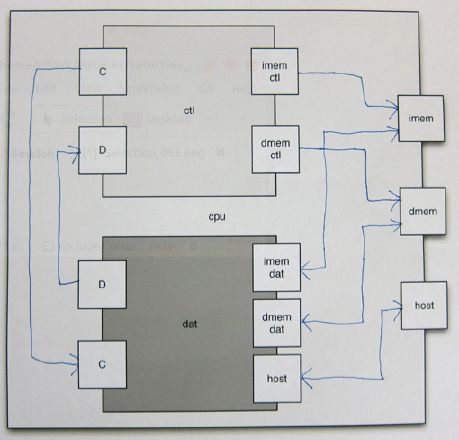
\includegraphics[width=\linewidth]{Bulk.png}
	
	作为铺垫,比如现在已有如下Chisel代码:
	\begin{scala}
class RomIo extends Bundle {
	val isVal = Input(Bool())
	val raddr = Input(UInt(32.W))
	val rdata = Output(UInt(32.W))
}
class RamIo extends RomIo {
	val isWr = Input(Bool())
	val wdata = Input(UInt(32.W))
}

class CpathIo extends Bundle {
	val imem = RomIo().flip()
	val dmem = RamIo().flip()
	...
}

class Cpath extends Module {
	val io = IO(new CpathIo())
	...
	io.imem.isVal := ...
	io.dmem.isVal := ...
	io.dmem.isWr := ...
	...
}
class Dpath extends Module {
	val io = IO(new DpathIo())
	...
	io.imem.raddr := ...
	io.dmem.raddr := ...
	io.dmem.wdata := ...
	...
}
	\end{scala}
	这里用的也是面向对象的技巧来尽可能的复用代码。这样如果要编写一个将这些模块连接起来的顶层模块,Verilog肯定是一大堆的端口,然后是一大堆的信号,但是用Chisel语言,就可以简化为:
	\begin{scala}
	class Cpu extends Module {
		val io = IO(new CpuIo())
		val c = Module(new CtlPath())
		val d = Module(new DatPath())
		c.io.ctl <> d.io.ctl
		c.io.dat <> d.io.dat
		c.io.imem <> io.imem
		d.io.imem <> io.imem
		c.io.dmem <> io.dmem
		d.io.dmem <> io.dmem
		d.io.host <> io.host
	}
	\end{scala}
	这种写法在Chisel的术语里叫做Bulk Connections。
	
	那么上面两个例子所体现出的语言特性有没有实际工程上的作用,当然有。一个最为典型的例子就是AXI接口,首先AXI是有五个通道,而且非常的规整。所以抽取出五个通道的共通之处,写出一个基类。然后对五个通道如果有多余的端口可以扩展这个基类,只需要添加多余的端口就行了。更妙的是,不同组件通过AXI总线共连时,用bulk connection的写法,每连一对总线,只需要写一行代码。
	
	Chisel的威力还不止于此,再举一个例子,如果要实例化多个同样的module,Chisel可以用for loop,但是Verilog也可以做到,那就是generate的写法。但是如果仔细一看,Chisel的for loop翻译为
	Verilog可不是用generate的写法,而是有几个实例化几个。一开始觉得这个是笨方法,但是后来发现这是个很明智的选择。首先这些都是Chisel编译器干的事情,一点都没有增加人的工作负担,不用复制粘贴。其次这种写法的好处就是更加通用。这个更加通用体现在万一需求是要实例化多个略有差别的不同配置的module,比如前面的第一个例子我要实例化100个不同功能的Filter,generate的写法显然不能胜任,但是Chisel编译的手法就能在for loop里面实现配置。然后编译好的Verilog文件真的就有100个不同配置的Filter。
	
	\subsubsection{Chisel test}
	沿袭了Verilog的传统,同一个语言可以用来设计电路也可以用来仿真电路,这样就不需要在两种语言之间做切换。由于Chisel承袭了Scala,而Scala承袭了Java,所以test设计的哲学思想也就自然顺承Java。从发展的角度来看,一开始的C\&C++没有严格的代码组织格式,test的设计也是如此,而且调试主要以真实的应用场景加上单步调试的GDB为主。到后来的Java对于代码的组织格式有了严格的要求,同时test的设计同样跟着代码的组织格式对每个模块进行了用例的assert测试。从而提出了一种比较系统的测试方法。引进的原因在于,用GDB跟着一个大系统单步调试往往效率是低下的,而把大系统拆分成一个个小的零件(其实也不用拆分,因为代码的组织格式就是按照一个个小的零件组织的),然后用一些包含edge case的用例来进行assert的测试就已经足够。这是一个非常好的想法,以至于后面的python更是凭借着解释语言的优势,可以以交互的方式对小零件单独测试,从而减少有这些小零件拼成的大系统的出bug数量和概率。所以Chisel自然有承袭了这一测试哲学。同时相比于Verilog中繁琐的测试代码编写,Chisel做了相应的简化与核心抽取。最大的一点改变就是不同于Verilog,在Chisel中不需要明确写出advance时钟一拍的逻辑,只需要简单写一句step(1)就能更新寄存器以及由寄存器驱动的组合逻辑。
 	\subsubsection{sbt build environment}
 	和Scala配套的build编译环境,和Java的maven类似,但其设计理念对于开发者更加友好。同时sbt种编译的依赖关系,比如Chisel的库。
	\subsubsection{Firrtl}
	作为编译系统里面最重要的一层--Intermediate Representation。事实上,要理解Chisel的运行机制,确保生成的电路万无一失,如果直接看由Chisel生成的近似于Netlist的Verilog,是unreadable的。而且生成的Verilog是slow to simulate。所以Chisel快速的仿真是基于Firrtl的。
	\begin{commentary}
		FIRRTL represents the standardized elaborated circuit that the Chisel HDL
		produces. FIRRTL represents the circuit immediately after Chisel’s elabora-
		tion but before any circuit simplification.
		
		FIRRTL has first-class support for high-level constructs
		such as vector types, bundle types, conditional statements, partial connects,
		and modules. These high-level constructs are then gradually removed by a
		sequence of lowering transformations. During each lowering transformation,
		the circuit is rewritten into an equivalent circuit using simpler, lower-level
		constructs. Eventually the circuit is simplified to its most restricted form,
		resembling a structured netlist, which allows for easy translation to an out-
		put language (e.g. Verilog). This form is given the name lowered FIRRTL
		(LoFIRRTL) and is a strict subset of the full FIRRTL language
	\end{commentary}

\section{ISA}
设计一款具体的CPU,就要考虑到具体基于哪一个ISA。好在RISC-V和MIPS非常相似,所以实现了一个,另外一个很多功能部件都能够复用。如果一开始的设计就是尽可能的将微结构和ISA接耦合,那么只需要修改少量的逻辑即可。所以计划是先实现RISC-V,然后在移植到MIPS。架构是32位。
\subsection{MIPS}
一个最为熟悉但却依旧陌生的ISA。熟悉的部分是MIPS 32中的整数指令部分,以及CP0寄存器堆和特权模式处理机制。但是囿于最初并没有考虑到64位的需求和嵌入式系统压缩指令长度的需求,导致指令空间设计考虑不周,使得日后出现的MIPS 64和microMIPS完完全全是不同的指令集,这是一个承重的历史包袱。所以MIPS的这些部分以及浮点部分对我来说是陌生的。
\subsection{RISC-V}
RISC-V作为一个2010年以后才出现的ISA,完全有着历史经验的优势,可以充分的借鉴前人设计的优缺点。所以32位,64位,压缩变长指令集都是统一的一个指令集下的不同形式。ISA的演进已经有40多年的历史,就目前而言逐渐趋向于收敛,而且RISC-V设计时也考虑到要有极强的可拓展性以便日后之需。同时RISC-V的设计模式也和之前所以增量式指令集不同:
\begin{quote}
	Unlike almost all prior ISAs, it is modular. At the core is a base ISA, called RV32I, which runs a full software stack. RV32I is frozen and will never change, which gives compiler writers, operating system developers, and assembly language programmers a stable target. The modularity comes from optional standard extensions that hardware can include or not depending on the needs of the application. This modularity enables very small and low energy implementations of RISC-V, which can be critical for embedded applications. By informing the RISC-V compiler what extensions are included, it can generate the best code for that hardware.
\end{quote}
那么相比于MIPS,RISC-V有什么特点呢?
\begin{enumerate}
	\item 首先自然是用户态指令和conversion的设计的对比。
	
	MIPS有延迟槽这么一条设计。这个被后来证明不是一个好主意,因为其设计的哲学就有问题,延迟槽实际上代表着ISA和设计实现的不独立,这是非常糟糕的。比如单发射五级流水有延迟槽就非常nice,不用停流水或者做转移猜测。但是对于多发射的实现呢?一条延迟槽不够了。这就是ISA和设计实现不独立的后果。在其他细节上,RISC-V取缔了HILO,但是32位的乘法和除法结果都是64位的,怎么解决。代码上写两条指令,一条得到低(商)32位,一条得到高(余数)32位,存在两个不同的寄存器里。那么这个设计有没有设计与ISA不独立之嫌呢?我觉得没有,首先在32位的架构下,寄存器都是32位的,如果要用到乘除法的结果,也是要通过mfhi,mflo指令来操作的。既然如此ISA就规定要算出乘除法的完整结果,就是需要两条指令,至于微结构实现要怎么做,那就看微结构的设计者,可以老老实实算两次,也可以一旦发现有连续的两条算高低位的指令,就做一次运算。如果恰好碰到中断之类的,就只好自认倒霉,再算一次了。同时算术指令中也取缔了overflow例外,将其移到了软件实现。在RISC-V中较于MIPS还有两大亮点:
	\begin{itemize}
		\item 不像MIPS用LWL,LWR来支持地址的非对齐访问。由于RISC-V指令可以是变长的,所以非对齐的访问是自然支持的。
		\item 
	\end{itemize}
\end{enumerate}
% \section{RTL model and logic}

% \subsection{instruction fetch}

% \subsection{branch prediction}

% \subsection{multi-issue \& out-of-order pipeline}

% \subsection{memory system}

% \subsubsection{load \& store mechanism}

% \subsection{precise exception handling}

% \subsection{the design which decouples microarchitecture and ISA}

% \subsection{referable instances}

% \subsubsection{Alpha 21264}
% \subsubsection{BOOM}

% \section{debug and verification}

% \section{Linux port}

% \section{multi-microprocessor support}

% \section{MPIS generator}

% \section{design space analysis and optimization}


\begin{thebibliography}{50}
\bibitem{chisel-dac12} Bachrach, J., Vo, H., Richards, B., Lee, Y., Waterman,
  A., Avi\v{z}ienis, Wawrzynek, J., Asanovi\'{c} \textsl{Chisel:
    Constructing Hardware in a Scala Embedded Language}.
in DAC '12.
\bibitem{gel} Bachrach, J., Qumsiyeh, D., Tobenkin, M. \textsl{Hardware Scripting in Gel}.
in Field-Programmable Custom Computing Machines, 2008. FCCM '08. 16th.
\end{thebibliography}

\end{document}
